\section{Analysis} \label{sec:analysis}
The analysis section will be split into different segments: Container technology, Kubernetes, the IoT/edge stack, and, finally, the requirements for the implementation. Essentially, the analysis will be the foundation of the implementation giving reason to the major design choices described in the requirements. The critical areas for the edge are: memory and disk space constrains, security, speed, protocols, loadbalancing and internet access.\\
In this thesis I will deploy containers to the edge using Kubernetes to determine what is still missing and what features already enable Kubernetes to make this possible. Standardization of the edge is going to be key.

% \subsection{Containers}
Containers first surfaced in 2007 with the release of Linux Containers (LXC). They provide an abstraction and isolation layer to the software they are supposed to run. Basically, a container is packaged software that runs independent from the underlying system. They are created at runtime from container images, which are packaged, standalone executable software including everything the main application needs to run (code, runtime, system tools, libraries and settings)\cite{containerDefinition:online}. Since 2007, there has been considered development of containers, especially by Docker, a company developing the same named application which is often used synonymously for containers. Docker than donated its main container runtime environment, called containerd, to the open source community and later, in late 2017, announced the first major release of containerd. https://blog.docker.com/2017/12/cncf-containerd-1-0-ga-announcement/ This was significant news, as the docker software was already widely used and it marked the start of an independent open source standard for containers. \\
Today, containers are the building blogs of the cloud and power almost all distributed applications. Craig McLuckie, the lead product manager cloud computing product at Google, said in a panel discussion during the Linux collaboration summit in Febraury 2015:
\begin{displayquote}
\textit{\textbf{\large{``}}}
\textit{This containers revolution is changing the basic act of software consumption. It’s redefining this much more lightweight, portable unit, or atom, that is much easier to manage... It’s a gateway to dynamic management and dynamic systems.}
\textit{\textbf{\large{''}}}
\end{displayquote}
It is important to note, that while the cloud saw the first transformation from containers the edge is part of the same dynamic system and also needs dynamic management.\\ 
The rest of the section will discuss the advantages of using containers focusing on the edge component. I will show the advantages and disadvantages of containers in terms of memory management, portability and security, and ways to combat the disadvantages. To keep the thesis concise I will not explain how containers in greater detail\footnote{For more information on this topic see Docker's website  \url{https://www.docker.com/resources/what-container} and containerd \url{https://containerd.io/}} .

\subsubsection{Resource consumption}
Memory consumption from containers is always greater than bare metal deployments. By design containers share little with the default namespace, apart from system resources, like the kernel. It is possible to give containers access to host directories, but this often breaks their design philosophy of being stateless and portable. The solution is to include the libraries, tools, certificates necessary to run the application in the container itself. It is not hard to image with multiple containers memory and RAM consumption can easily exceed the system resources of edge devices, e.g. the Raspberry Pi’s. For example, deploying the latest official openJDK container consumes 470MB. Source and byte code and dependencies add on top of this. Compiled language are at a huge advantage in this regard. Go is one such example and used in this thesis. It can be cross-compiled to machine code for most CPU architecture compatible with Linux and results in one application file without any dependencies. Multi-stage builds allow to have one container to build the application and only copy relevant files into the final image. This eliminates any unused files and is often used in combination with the \textit{scratch} image. This is the base image for all other containers and is basically an empty file structure consuming no memory. According to Docker it ``is most useful in the context of building [...] super minimal images''\cite{scratchImageDockerD65:online}.\\
Combining these these techniques can result in far lower memory and RAM consumption, but also better security (discussed in the next section). In the implementation, \cref{sec:testService} \nameref{sec:testService}
hard topic, as this is not needed in the cloud
\subsubsection{Security}
Security is one of the biggest challenges in IoT. In 2016 a botnet with over 600k infected devices, primarily edge and IoT devices, overwhelmed several high-profile targets like the DNS provider Dyn with massive distributed denial-of-service (DDoS) attacks. This caused a temporary outage of their DNS servers rendering many webpages, among others  Twitter, Spotify and Amazon, temporally inaccessible. To combat malicious attacks certain methods have been developed. I will only analyze the direct container security aspects as they are always applicable for containers. Other methods, like specifically developed OSs and securing the CI/CD pipeline are not discussed at this point.\\
Most registries allow for overriding of images. In the implementation \cref{sec:testService} \nameref{sec:testService} I will use the \textit{hello} service for testing. It's current version, v5arm, is saved on the Docker image hub and can be pulled with the link \textit{jonas27/hello:v5arm}. However, each image also has an image digest, a cryptographic signature ensuring that the image in question is the actual image. In production (not done in this thesis) an image should always be pulled based on the image digest, also called "Pinning-by-Digest". In the case of the test service the link would then be \textit{jonas27/hello:sha256:725355347bc2eae8f7c9ab9dd09b9ef2c884b3458c693978f5408785aef1fb72}. This simple technique not only improves security but also guarantees that each container is derived from the same image, but it also guarantees that every instance of the service is running exactly the same code and combats race conditions.\\
In a recent talk at the "Container Security Conference" Andy Martin, co-founder of control plane, noted ``The root of all evil is unnecessarily running processes or containers as root''\cite{RootlessContainerSecurityTalk0:online}. By default, all images use the root user as default user. However, the root user can read, write and run all files in all directories. In the beginning of 2018 a new vulnerability on Kubernetes was discovered giving containers with volume mounts the ability to access data outside the volumes sub-path. The root user would thus have unlimited access to the host resources. To combat this, the user can be changed to a newly created user. 

Scratch user
binary no reverse engineering
no modification possible.



\comment{
https://www.iotforall.com/containers-on-the-edge/

 They isolate the application runtime and the 

Containers and Cloud: From LXC to Docker to Kubernetes

}

% \subsection{Kubernetes}
Kubernetes is the de-facto standard for container orchestration and the main aspect of this thesis. In this section I look at the fundamentals of Kubernetes and highlight the best strategies to run it on edge devices. I will also look what is currently missing to make it a truly edge ready. With that being said, Kubernetes has so many features and tools that discussing them all is impossible. The same is true for its ecosystem which is constantly evolving and adding even more layers to the mix. I will try to keep this section short and concise, but it will come at the cost of complexity.\\
IIoT has accelerated the need for fog computing and the industry is set to develop a container based orchestration tool, tightly integrated with Kubernetes. The Kubernetes IoT edge working group was set up specifically to find the optimal Kubernetes strategy for the edge. However, it is not clear, whether the solution will be Kubernetes itslef or a more specialized tool. In this thesis I will argue that Kubernetes is the way forward as it already posses many of the features that are need for the edge.\\ 
I will start with addressing the elephant in the room, single-cluster vs multi-cluster. I will then analyze the core components of Kubernetes, mainly the kubelet, together with other resource configurations. Afterwards, I will focus on the optimal deployment strategy, how to control resources on the edge and node selection. Finally, I will look at the security aspect of Kubernetes and conclude with recommendations for the implementation.

\subsubsection{Single Vs Multi-Cluster}
Google recently revealed a new and much hyped product, Anthos\cite{TechnicalAnthosGoogle66:online}. Its a combination of many services, but most importantly it lets people easily manage hybrid clouds. Google describes it as follow: "Anthos is a modern application management platform that provides a consistent development and operations experience for cloud and on-prem environments"\cite{TechnicalAnthosGoogle66:online}. Google provides an installer for on-prem but onece installed Google itself manages the cluster including updates and troubleshooting. Not only is it a multi-cluster solution, but it also integrates the clusters with Istio service mesh and other neat features. Open source Kubernetes only has the multi-cluster management solution called Kubernetes Cluster Federation.



\subsection{The IoT/Edge Problems}
Resource consumption and orchestration are big problems in the cloud and equally so for the edge. Containers and Kubernetes can be adopted to consume less resources and Kubernetes enables remote orchestration of on-prem nodes. But, because of the heterogeneity of the edge, it faces even more problems. Discussed in this section will be load balancing, protocol conversion and traffic shaping.\\ Not thoroughly discussed in this section will be the issue of ultra low latency. In an updated performance assessments of containers the authors found that containers introduce almost no overhead over a native deployment\cite{felter2015updatedPerformanceContainers}. Hence, gateways running Linux can in most cases use containers without a problem. 

\subsubsection{Load Balancing}
Load balancing in a distributed environment is difficult as the ingress node needs a complete network topology at any given moment in time. This is one of the reasons why Kubernetes refreshes its node status so often. If a external request comes in at the master it needs to know where to forward the traffic. In the previous section \cref{sec:singleVsMultiCluster} \nameref{sec:singleVsMultiCluster} I discussed the advantages and disadvantages of multi-cluster in contrast to single clusters and load balancing is a perfect example why the decision has to be carefully weight. A full Kubernetes cluster on the edge comes with the advantage of having a full control plane on the edge and, thus, being able to do load balacing on the edge, with for example Istio Ingress Gateay. If the master nodes taint were to be removed it could even become part of the operational unit of the cluster.\\
But having a cluster at edge comes with its downside. It needs a lot more management than a single cluster setup. It consumes drastically more resources than having only worker nodes and it needs a stable connection between the cluster nodes to work. But if resource consumption on the master is not an issue Kubernetes coupled with a load balancer provide more features and safeguarding than most other load balancers do. Kubernetes always ensures that pods inside the cluster are healthy and reachable and if a pod goes down, Kubernetes will automatically spawn a new one. The internal load balancer can use this information and always route to an available pod. Other gateways like, Kong API Gateway, can not do this. Also with Istio it becomes possible to do very fine grained traffic routing, somthing I will discuss in the next section \cref{} \nameref{}.\\
Finally, internal load balancing\footnote{Load balancing withing one node.} is possible through normal API gateways and the deployment of multiple pods listening on different ports. For example, one NGINX container could function as load balancer for 5 docker containers in the background. In Kubernetes this could be solved with affinities. As soon as a node runs certain pods, a load balancer could be automotically side loaded.
\subsubsection{Traffic Control and Shaping}
Traffic control and traffic shaping are very interesting edge topics. In Kubernetes each pod can be assigned incoming and outgoing bandwidth rates. But other tools extend this functionality and open up new possibilities. Istio, a service mesh mainly developed for Kubernetes, injects a sidecar proxy to fine tune the traffic of each container. It makes it possible to do rate limiting, control headers, reroute connection, change retries attempts, circuit breaking, mirroring and more while not changing the application code. Additionally, it is also able to encrypt traffic inside the mesh without the application knowing about it and gather all the telemetry data of the cluster. \\
With Kubernetes and tools extending its capabilities it is possible to do both traffic control and traffic shaping on a fine grained level. But, especially Istio, comes at the cost of additional overhead and the operator has to decide if the added functionality are worth the performance hit. Without Istio traffic control and shaping is only possible through the Kubernetes Ingress and thus in multi-cluster solutions.\\
Finally, Kubernetes is only meant to work with the Internet protocol stack and is only meant to operate within the clusters boundaries. So the actual communication with the IoT devices can not be controlled or shaped with Kubernetes. 
\subsubsection{IoT Protocols and Protocol Conversation}
Kubernetes was designed for the Inernet and not for the heterogenity of the edge. This means the IoT gateway must either implement a DHCP server, the IoT device must have a static IP or the communication is facilitate outside Kubernetes realm and then converted by a service to IP. Please note that lower level protocols for establishing a connection between two devices, e.g. Ethernet, Wi-Fi (IEEE-802.11) or Bluetooth, are not discussed at this point. The most common IoT protocols are MQTT, CoAP, AMQP and DDS. In contrast to Internet protocol stack, these technologies do not need to support legacy systems and can thus concentrate on whats important in IoT, very low energy, distribution and memory consumption. I will mainly compare MQTT\cite{MQTT50:online} to CoAP\cite{CoAP—Con75:online} because of the their vast usage and academic literature. \Cref{fig:mqttVsCoap} shows side by side the architecture of MQTT and CoAP. Both are based on machine to machine (m2m) communication and are optimized for the IoT space, but the similarities stop there.
\begin{figure}[h!]
    \centering
    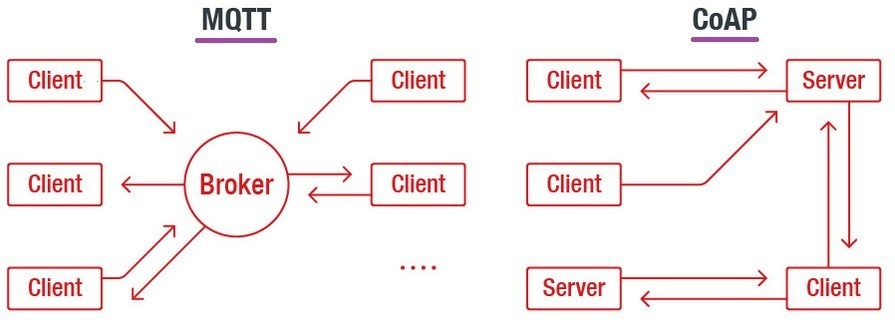
\includegraphics[scale=0.45]{figures/mqtt-vs-coap.jpg}
    \caption{MQTT and CoAP architecture side by side\cite{COAPvsMQTT27:online}.}
    \label{fig:mqttVsCoap}
\end{figure}
MQTT is based on the publish-subscribe massaging pattern which relies on a central entity, called broker, to enable communication between multiple nodes, mainly IoT devices. CoAP on the other side is a classic client server protocol and is based on the Internet stack. Researches compared the two standards and found "MQTT messages experienced lower delays than CoAP for lower packet loss and higher delays than CoAP for higher packet loss"\cite{MQTTvsCoAPAnalysisIEEE}. They also found that the message overhead for small messages is significantly lower at 25\% or less for CoAP compared to MQTT for reliable message transmission. Whereas in MQTT the broker needs additional services to convert the data to Internet compatible standards, CoAP is already able to communicate directly through the Internet. This opens up new possibilities including decentralized communication in subnets.\\
Finally, the data serialization can be even more important than the protocol itself. With the advent of RESTful services JSON soared in popularity. It is human readable but not very space efficient. When researches compared JSON to protobufs they found huge message size differences between the two, shown in \cref{fig:jsonVsProtobufs}.
\begin{figure}[h!]
    \centering
    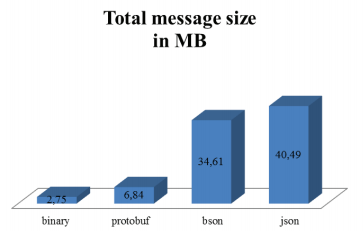
\includegraphics[scale=0.45]{figures/jsonVsProtobufs.png}
    \caption{Memory consumption of different serialization methods\cite{}.}
    \label{fig:jsonVsProtobufs}
\end{figure}
The researches conclude "the Protocol Buffers are a serious candidate for standardized way of communication in field of Internet of Things"\cite{jsonVsProtobufs}.

\comment{
protocol conversation
Traffic shaping
Load balacing
}







\comment{In fact, a new Kubernetes IoT Working Group is investigating how it can provide a consistent deployment model for IoT cloud and IoT Edge.
https://blog.bosch-si.com/bosch-iot-suite/why-the-iot-needs-kubernetes/

WHTA is important for edge? 
small containers
internet access (function without)
security
Speed (kubelet)
protocols


}